\documentclass{article}
\usepackage{pdfsync}
\usepackage{fullpage}
\usepackage{natbib}


% custom %
\usepackage{amsmath,amsthm,amssymb,xspace,amsfonts}
\usepackage{mathtools}
\usepackage{xcolor}
\usepackage[]{algorithm}
\usepackage{fancyhdr}
\usepackage{bbm}
\usepackage{enumitem}
\usepackage{graphicx, subfig}
\usepackage{caption}

\usepackage{cleveref}
\usepackage{thm-restate}
\usepackage{listings, pdfpages}
\usepackage[T1]{fontenc}
\usepackage{algpseudocode}
\usepackage{subfiles}

\newcommand{\vect}{\mathbf}
\newcommand{\cc}[1]{\ensuremath{\mathsf{#1}}}
\newcommand{\algprobm}[1]{{\sc #1}\xspace}

\newcommand{\E}{\mathbb{E}}

\newcommand{\K}{\mathcal{K}}
\newcommand{\lt}{\ell_t}
\newcommand{\glt}{\nabla \ell_t}
\newcommand{\sumt}{\sum_{t=1}^T}
\newcommand{\sumk}{\sum_{i=1}^k}

\newcommand{\xs}{x^*}
\newcommand{\xst}{x^*_t}


\newcommand{\tildegt}{\tilde{g}_t}
\newcommand{\proj}[2][]{\textit{proj}_{{#1}}{#2}}


\newcommand\tab[1][0.5cm]{\hspace*{#1}}

\theoremstyle{definition}
\newtheorem{defn}{Definition}
\newtheorem{theorem}{Theorem}
\newtheorem{lemma}{Lemma}
\newtheorem{proposition}{Proposition}
\newtheorem{assumption}{Assumption}
\newtheorem{corollary}{Corollary}
\newtheorem{claim}{Claim}

\newtheorem*{problem}{Decision Problem}

\newenvironment{claimproof}[1]{\par\noindent\underline{Proof:}\space#1}

\newenvironment{pfsketch}[1]{\par\noindent\underline{Proof sketch:}\space#1}

\DeclarePairedDelimiter\abs{\lvert}{\rvert}%
\DeclarePairedDelimiter\norm{\lVert}{\rVert}%

\DeclarePairedDelimiter\ceil{\lceil}{\rceil}
\DeclarePairedDelimiter\floor{\lfloor}{\rfloor}

% Swap the definition of \abs* and \norm*, so that \abs
% and \norm resizes the size of the brackets, and the 
% starred version does not.
\makeatletter
\let\oldabs\abs
\def\abs{\@ifstar{\oldabs}{\oldabs*}}
%
\let\oldnorm\norm
\def\norm{\@ifstar{\oldnorm}{\oldnorm*}}
\makeatother


\newlength\myindent
\setlength\myindent{2em}
\newcommand\bindent{%
	\begingroup
	\setlength{\itemindent}{\myindent}
	\addtolength{\algorithmicindent}{\myindent}
}
\newcommand\eindent{\endgroup}


\algrenewcommand{\algorithmiccomment}[1]{\hskip3em$\vartriangleright$ #1}

\newcommand{\dk}[1]{\textcolor{red}{[DK: #1]}}
\begin{document}

\title{Between Bandit and Full-Information: Regret bounds for Online Gradient Descent}
 \author{Dhamma Kimpara}

\maketitle


\section{Introduction}\label{sec:intro}
\begin{defn}
	Regret:
	$$\E \frac{1}{k} \sumt \sumk \lt(y_{t,i}) - \E \sumt \min_{\xst\in \K}\ell_t(\xst)$$
\end{defn}




\section{Preliminaries}

\subsection{Problem Setting}

First we formally introduce the problem. Our objective is:

\[\min_{x_t \in \mathcal{K}} \ell_t(x_t)\]

over rounds $t=1,\dots, T$. Where $\K \subset \mathbb{R}^d$ is our action set and $\ell_t$ are adversarially chosen time varying loss functions. The key in our setting is that we do not have first order gradient information $\glt$ but we are able to get zeroth-order (bandit) feedback with $k=d+1$ points. First we outline our assumptions.

We assume that $\K$ is compact and has a nonempty interior (otherwise project $\K$ to a lower dimensional space). For this work, when we implicitly or explicitly refer to norms, we will be using the euclidean norm. We also have the following assumptions for each loss function $\lt$:

\begin{assumption}
	Let $\mathcal{B}$ denote the unit ball centered at the origin. There exists $r,D > 0 $ such that
	\[r \mathcal{B} \subseteq \K \subseteq D \mathcal{B}\]
\end{assumption}

\begin{assumption}
	Strong Convexity. For $\mu \geq 0$, $\ell_t$ is $\mu$-strongly convex over the set $\K$:
	\[\ell_t(x) \geq \lt(y) + \nabla \lt(y)^\intercal(x-y) + \frac{\mu}{2} \norm{x-y}^2, ~~ \forall x,y \in \K\]
\end{assumption}

\begin{assumption}
	$\lt$ is $L$-smooth on $\K$ if it is differentiable on an open set containing $\K$ and its gradient is Lipschitz continuous with constant $L$:
	\[\norm{\glt(x)-\glt(y)} \leq L \norm{x-y}, ~~ \forall x,y \in \K\].
\end{assumption}


\begin{assumption}
	$\lt$ is G-Lipschitz:
	\[\norm{\lt(x)-\lt(y)} \leq G \norm{x-y}, ~~ \forall x,y \in \K\].
	
	Hence the gradient of $\ell_t$ over $\K$ is bounded:
	\[\norm{\nabla \ell_t(x)} \leq G ~~ \forall t, \forall x \in \K\]
	
\end{assumption}


We also use the notation $\E_t$ to denote the conditional expectation conditioned on all randomness in the first $t-1$ rounds. 



\section{Projected Gradient Descent with $k$ queries per round}
\begin{algorithm} 
	\begin{algorithmic}
		\caption{Generic $k$-point Bandit Online Gradient Descent }\label{alg:generic}
		\State \textbf{Input:} Step size $\eta$, exploration parameter $\delta$ and shrinkage coefficient $\xi$.
		\State Set $x_1 = 0$
	
		\For{$t = 1, ..., T$} 
			\State Observe randomized queries around $x_t$: $\lt(y_{t,1}), \dots, \lt(y_{t,k})$ 
			\State Estimate the gradient $\tildegt = g(\lt(y_{t,1}), \dots, \lt(y_{t,k}))$.
			\State Update $x_{t+1} = \proj[(1-\xi)\K]{(x_t - \eta \tilde{g}_t)}$.
		\EndFor

	\end{algorithmic}
\end{algorithm}\newpage

In this section we present a no-regret result for any algorithm that is an instantiation of Algorithm \ref{alg:generic} for some $k$ and where its randomized gradient estimate satisfies boundedness and closeness of its expectation to the true gradient. We assume the reader is familiar with OGD.

We first explain the algorithm. It plays $k$ actions, constructs a gradient estimate $\tildegt$ from its $k$ actions in round $t$ and performs the OGD step to produce the next action $x_{t+1}$:

$$x_{t+1} = \proj[(1-\xi)\K]{(x_t - \eta \tilde{g}_t)},$$

where $\xi \in (0,1)$ and $(1-\xi)\K$ is shorthand for $\{(1-\xi)x : x \in \K\}$. Note that our gradient estimators will randomly query around the action $x_t$ in order to estimate the gradient. Thus the projection is made onto the shrunk set to ensure that the random queries around the point $x_{t+1}$ belong to $\K$. For any $x \in (1-\K)$ and any unit vector $u$ it holds that $(x+\delta u ) \in \K$ for any $\delta \in [0, \xi r]$ \citep{flaxman2004online}. 




We now present the main result. But first, we need two Lemmas the first is the dynamic regret bound of OGD and the second is the difference in regret between playing $x_t$ on $\K$ and $\{y_{t,i}\}_{i=1}^k$ on $(1-\xi) \K$.
\dk{check $\eta$}
\begin{lemma} \citep{mokhtari2016online}.\label{lem:OGD}
	Assume that the functions $h_t$ are strongly convex and $L$-smooth. Assume further that the gradient norms are bounded and the step size is chosen such that $\eta \leq 1/L$. Then, the dynamic regret $Regret_T^d$ for the sequence of actions $x_t$ generated by OGD is bounded by
	
	$$Regret_T^d(OGD, G):= \sumt h_t(x_t) - \sumt \min_{\xst\in \K} h_t(\xst) \leq G K_1 \sum_{t=2}^T \norm{\xst - x_{t-1}^*} + G K_2$$
	
	where the constants $K_1$ and $K_2$ are explicitly given by
	
	$$K_1 := \frac{\norm{x_1 - x_1^*} - \rho \norm{x_T - x_T^*}}{(1-\rho)}, ~~ K_2 := \frac{1}{1-\rho}.$$
	
	Where $0 \leq \rho := (1-\eta\mu) ^ {1/2} < 0$. Is our linear convergence constant.
\end{lemma}

\begin{lemma} \label{lem:2}
	For any point $x \in \K$,
	
	$$\frac{1}{k} \sumk \lt(y_{t,i}) - \ell_t(x) \leq  \lt(x_t) -  \lt((1-\xi)x) + G\delta + GD\xi.$$
	
\end{lemma}
 
\begin{proof}
	By assumption of Lipschitz continuity,
	
	$$\lt(y_{t,i}) \leq \lt(x_t) + G \delta.$$
	
	We also have that by the Lipschitz property and $\norm{x} \leq D$, for all $x \in \K$,
	$$\lt((1-\xi)x) \leq \lt(x) + GD\xi.$$
	
	Combining the above two inequalities we get
	$$\frac{1}{k} \sumk \lt(y_{t,i}) + \lt((1-\xi)x) \leq \lt(x_t) + \lt(x) +  G \delta + GD\xi.$$
	
	Rearranging terms gives us the Lemma.
	
	
\end{proof}


\begin{theorem} \label{thm:one}
	Suppose the assumptions in the preliminaries hold. Suppose on round $t$ the algorithm plays $k$ random queries $y_{t,1}, ..., y_{t,k}$, constructs a gradient estimator $\tilde{g}_t = g(y_{t,1}, ..., y_{t,k})$ and uses the the algorithmic step $x_{t+1} = \proj[(1-\xi)\K]{(x_t - \eta \tilde{g}_t)}$ with $\eta \leq \frac{1}{2G_1}$, $\delta = \frac{\log(T)}{T}$, and $\xi = \frac{\delta}{r}$. If the gradient estimator satisfies the following conditions for all $t \geq 1$:
	
	\begin{enumerate}
		\item $\norm{x_t - y_{t,i}} \leq \delta \text{ for } i = 1, ... k$.
		\item $\norm{\tildegt} \leq G_1$ for some constant $G_1$.
		\item $\norm{\E_t \tildegt - \glt(x_t)} \leq c\delta$ for some constant $c$. 
		 
	\end{enumerate}
	Then for any sequence $\{\xst\}_{t=1}^{T}, \xst\in\K$ we have
	
	$$\E \frac{1}{k} \sumt \sumk \lt(y_{t,i}) - \E \sumt \min_{\xst\in \K}\ell_t(\xst) \leq G_1 K_1 \sum_{t=2}^T \norm{\xst - x_{t-1}^*} + G_1 K_2 + G \log(T)\big(1 + 2c + \frac{D}{r}\big).$$
	
	where the constants $K_1$ and $K_2$ are explicitly given by
	
	$$K_1 := \frac{\norm{x_1 - x_1^*} - \rho \norm{x_T - x_T^*}}{(1-\rho)}, ~~ K_2 := \frac{1}{1-\rho}.$$
	
	Where $0 \leq \rho := (1-\eta\mu) ^ {1/2} < 0$ is our linear convergence constant.
	

\end{theorem}


\begin{proof}
	Start by defining $h_t(x) = \lt(x) + (\tildegt - \glt(x))^\intercal x$. Then $h_t$ has the same convexity properties as $\lt$ and is $L_1$-smooth. Note also that $\nabla h_t(x_t) = \tildegt$. So we can pretend that the algorithm is actually performing deterministic gradient descent, as if with full information, on the functions $h_t$ restricted to $(1-\xi) \K$. Using the OGD regret bound from Lemma \ref{lem:OGD} we have that since $\nabla h_t(x_t) = \tildegt$ and hence $\norm{\tildegt} \leq G_1$ (So $h_t$ is $2G_1$-smooth since $\nabla h_t$ is $2G_1$-Lipschitz),
	 
	$$\sumt h_t(x_t) - \sumt h_t(\xst) \leq G_1 K_1 \sum_{t=2}^T \norm{\xst - x_{t-1}^*} + 2G_1 K_2 := Regret_{T}^d(OGD, G_1).$$ 
	
	Then taking expectations,
	
	\begin{align*}
		\E \sumt [\lt(x_t) - \lt(\xst)] &= \E \sumt [h_t(x_t) - h_t(\xst)] + \E \sumt[\lt(x_t) - h_t(x_t) - \lt(\xst) + h_t(\xst)] \\
		&\leq Regret_{T}^d(OGD, G_1) + \E \sumt (\E_t \tildegt - \glt(x_t))^\intercal(x_t - \xst)\\
		& \leq Regret_{T}^d(OGD, G_1) + 2c\delta DT.
	\end{align*}
	
	Where the first inequality is by the convexity of $\ell_t$ and $h_t$. Now we use Lemma \ref{lem:2} and obtain
	
	$$\E \frac{1}{k} \sumt \sumk \lt(y_{t,i}) - \E \sumt \min_{\xst\in \K}\ell_t(\xst) \leq Regret_{T}^d(OGD, G_1) + 2c\delta DT + TG\delta + GDT\xi.$$
	
	To finish the proof, plug in the values for $\delta$ and $\xi$.
	
\end{proof}






\begin{algorithm}
	\begin{algorithmic}
		\caption{\gscore$(\dtriple)$} \label{alg:gscore}
		\State \textbf{Input:} A Dodgson triple $\dtriple$.
		\State
		\For{$d \in C \setminus \{c\}$} \Comment Initialize counter variables
			\State $Deficit[d] \leftarrow 0$ \Comment Number of votes by which $c < d$ ($d$ beats $c$)
			\State $Swaps[d] \leftarrow 0$ \Comment Number of votes by which $c \prec d$ (greedily swappable votes against $d$)
		\EndFor

		\For{each vote $v \in V$} \Comment each vote is an 
		array where $v[k] \prec v[k+1]$
			\State $i \leftarrow 1$
				\While{$v[i] \neq c$}
					\State $d \leftarrow v[i]$
					\State $Deficit[d] \leftarrow Deficit[d]-1$
					\State $i \leftarrow i+1$
				\EndWhile
				\If{$ i < length(v)$}
					\State $d \leftarrow v[i+1]$
					\State $Swaps[d] \leftarrow Swaps[d]+1$
				\EndIf
				\For{$i \leftarrow i + 1$ to $length(v)$ }
					\State $d \leftarrow v[i]$
					\State $Deficit[d] \leftarrow Deficit[d]+1$


				\EndFor
		\EndFor
		\State $confidence \leftarrow$ ``definitely''
		\State $score \leftarrow 0$
		\For{$d \in C \setminus \{c\}$} \Comment If there are more than $1+Deficit[d]/2$ greedily swappable votes,
			\If{$Deficit[d]\geq 0$} \Comment then this is the Dodgson Score of $c$.
				\State $score \leftarrow score +
				\floor{Deficit[d]/2} + 1$ 
				\If{$Deficit[d] \geq 2 \cdot Swaps[d]$}
					\State $confidence \leftarrow$ ``maybe''
					\State $score \leftarrow score + 1$
				\EndIf
			\EndIf
		\EndFor
		\State \textbf{Output:} $(score,~confidence)$
	\end{algorithmic}
\end{algorithm}
\begin{algorithm}
\begin{algorithmic}
	\caption{\gwin$(\dtriple)$} \label{alg:gwin}
	\State \textbf{Input:} A Dodgson triple $\dtriple$ where
	we want to test whether $c$ is a Dodgson winner in the
	election.
	\State $(cscore,~confidence) \leftarrow \gscore(\dtriple)$
	\State $winner \leftarrow $ ``yes''
	\For{$d \in C \setminus\{c\}$}
		\State $(dscore,~confidence) \leftarrow
		\gscore(\langle C,d,V \rangle)$
		\If{$dscore < cscore$}
			\State $winner \leftarrow$ ``no''
		\If{$dcon = $ ``maybe''}
			\State $confidence \leftarrow$ ``maybe''
		\EndIf
		\EndIf
	\EndFor
	\State \textbf{Output:} $(winner,~confidence)$
\end{algorithmic}
\end{algorithm}
\section{$d+1$ point feedback}
In this section, we show that we can construct a deterministic gradient estimator using $d+1$ point feedback. Thus we obtain a deterministic version of Theorem \ref{thm:one}. Hence, the algorithm is no-regret even against completely adaptive adversaries meaning that the adversary can choose the loss $\lt$ after the algorithm plays $x_t$. Hence we match the full-information bound.

The algorithm constructs the deterministic gradient estimator
$$\tildegt = \frac{1}{\delta} \sum_{i=1}^{d} (\lt(x_t + \delta e_i)-\lt(x_t))e_i.$$

Where $e_i$'s are the standard unit basis vectors. We further need only the assumptions on strong convexity and $L$-smoothness, since they imply a bound on the gradient which we denote $G$. We can thus derive a bound on the norm of the estimator

\begin{align*}
	\norm{\tildegt} &= \norm{\frac{1}{\delta} \sum_{i=1}^{d} (\lt(x_t + \delta e_i)-\lt(x_t))e_i} \\
	& \leq \frac{d}{\delta} \max_i \norm{\lt(x_t + \delta e_i)-\lt(x_t)} \\
	& \leq \frac{d}{\delta} \delta G \\
	&= dG.
\end{align*}

And also the divergence of the estimator and the true gradient
\begin{align*}
\norm{\tildegt - \glt(x_t)} &= \sqrt{\frac{1}{\delta} \sum_{i=1}^{d} |(\lt(x_t + \delta e_i)-\lt(x_t))e_i - \langle \glt(x_t), e_i \rangle|^2} \\
& \leq %%use lipschitz \\
& \leq  \\
&= \frac{\sqrt{d} L \delta}{2}
\end{align*}

Hence we have that the properties of $\tildegt$ are the deterministic version of the properties of the estimator outline in theorem \ref{thm:one}. Hence we have an algorithm that can guarantee no-regret against a completely adaptive adversary. 


\begin{theorem} \label{thm:dplusone}
	Suppose a completely adaptive adversary chooses the sequence of loss functions $\{\lt\}_{t=1}^T$ subject to the same assumptions as above. If Algorithm \ref{alg} is run with the $1/\eta \geq L$, $\delta = \frac{\log(T)}{T}$, and $\xi = \frac{\delta}{r}$, then
	
	$$\sumt \frac{1}{d+1} (\lt(x_t) + \sum_{i=1}^{d}\lt(x_t+\delta e_i)) - \sumt \lt(\xst) \leq
	Regret_T^d(OGD) + G \log(T) \big(1 + \frac{\sqrt{d} L \delta}{2}
	+ \frac{D}{r}\big).$$
\end{theorem}

\begin{proof}
This is a modification of the proof of Theorem \ref{thm:one}. Define $h_t(x) = \lt(x) + (\tildegt - \glt(x))^\intercal x$. Then $\norm{\nabla h_t(x_t)} \leq dG$. Hence from Lemma \ref{lem:OGD} for any sequence $\{\xst\}_{t=1}^T$,

$$\sumt h_t(x_t) - h_t(\xst) \leq Regret_T^d.$$

Then we use $\norm{\tildegt - \glt(x_t)} \leq \frac{\sqrt{d} L \delta}{2}$. Apply Lemma \ref{lem:2} and plug in our parameters and this gives us the result.

\end{proof}


\section{Experiments}

In this section we present empirical results based on our
implementation the ~ algorithm from the previous section (see appendix for
the python code).
As proved in the previous section, the algorithm should succeed with high
probability when $n \sim \Omega(m^2)$ so we tested values for $n$ ranging between
$n = m^{1.5}$ to $m^{2.5}$ for each $m$ between 5 and 50.
For $m \in [50,100]$ we ran experiments for $n = m^{2.1}$ to $m^{2.5}$
Note that the experimental values for $m$ were not evenly spaced apart.
Each pair of $n,m$ was run for 100 trials, each trial consisting of generating
an election uniformly at random, picking a random candidate to test, and running ~ on that
instance.
A success was when returned ``definitely'', as in it was self-knowingly correct.

At 100 candidates, the 100 trials took 9 hours, while at 5 candidates, the trials
took about 3 minutes.


\begin{figure}[hbt!]\centering
    \subfloat{
    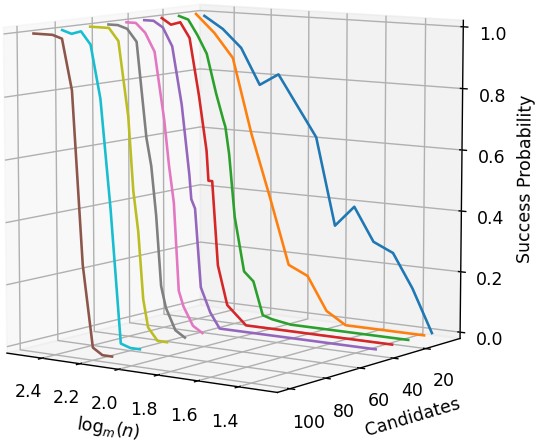
\includegraphics[width=0.45\linewidth]{gwinNoErr.png}}\hfill
    \subfloat{
    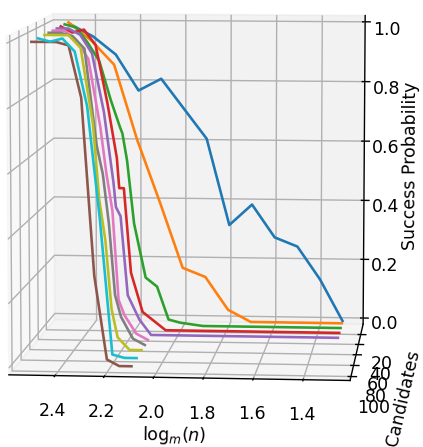
\includegraphics[width=0.45\linewidth]{view2.png}}
    \caption{3D line plot showing the success probability of the
    ~algorithm. Each line color corresponds to a particular
    number of candidates. 100 trials were run for each pair of $n,m$.
    Error bars were omitted to not clutter the graph. For reference they
    are at most $ 0.08$.}
    \label{fig:exp}
\end{figure}

Figure \ref{fig:exp} 





\newpage

\bibliographystyle{plainnat}
\bibliography{bib}

\newpage

\appendix

\section{Code}
\subsection{Algorithm}

\subsection{Data Collection}


\end{document}

%%% Local Variables:
%%% mode: latex
%%% TeX-master: t
%%% End:
